\begin{wrapfigure}{R}{0.45\linewidth}
\centering
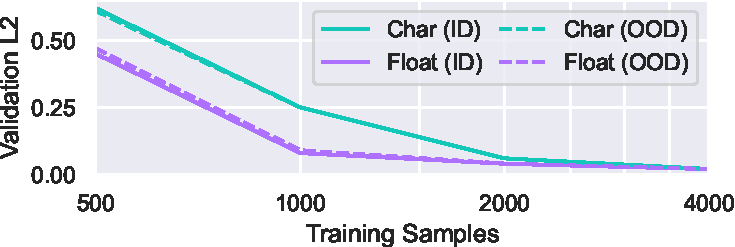
\includegraphics[width=\linewidth]{figures/clevr/data_efficiency_plot.pdf}
\caption{\textbf{CLEVR Data Efficiency.} (\cref{ssec:clevr})
Plot of the validation L2 positional error by the number of training samples.
We observe that the float-based model is consistently more data-efficient but that the difference between the models converges as the number of training samples reaches 4000.
See \cref{table:clevr_data_efficiency} for a full quantitative comparison.
}
\label{fig:clevr_data_efficiency}
\vspace{-0.5cm}
\end{wrapfigure}